\documentclass[11pt]{article}
%\usepackage[a3paper]{geometry}
%\usepackage[]{babel}
\usepackage[utf8]{inputenc}
\usepackage[T1]{fontenc}
\usepackage{fancyhdr}
\usepackage{graphicx}
\usepackage{amsmath}
\usepackage{amsfonts}
\usepackage{enumerate}
\PassOptionsToPackage{hyphens}{url}\usepackage{hyperref}
\usepackage {tikz}
\usetikzlibrary {positioning,fit,matrix,chains,calc,shapes.multipart,arrows,decorations.pathreplacing,shapes.arrows,chains,positioning}
\newlength\myht
\settoheight{\myht}{$n-2$}
%\usepackage{pgf}
%\usepgfplotslibrary{units}


\topmargin=0cm \oddsidemargin=0cm \evensidemargin=0cm \textheight=21cm
\textwidth=16cm \headheight=15pt \footskip=35pt

%\topmargin=0cm \oddsidemargin=0cm \evensidemargin=0cm \textheight=35cm
%\textwidth=25cm \headheight=15pt \footskip=35pt

\pagestyle{fancyplain}
\fancyhead{} % clear all header fields
\lhead{Enseirb-Matmeca M2 2021-2022}
\rhead{Quickly Différences Finies 2D}
\fancyfoot{} % clear all footer fields
\cfoot{\thepage}

\begin{document}

%headers
\begin{center}
{\bf \Large Quickly Différences Finies 2D } \\ 
N. Barral (\href{mailto:nicolas.barral@enseirb-matmeca.fr}{nicolas.barral@enseirb-matmeca.fr})
\end{center}
\hrule
\vspace*{1cm}

% beginning of the content


\begin{figure}[!ht]
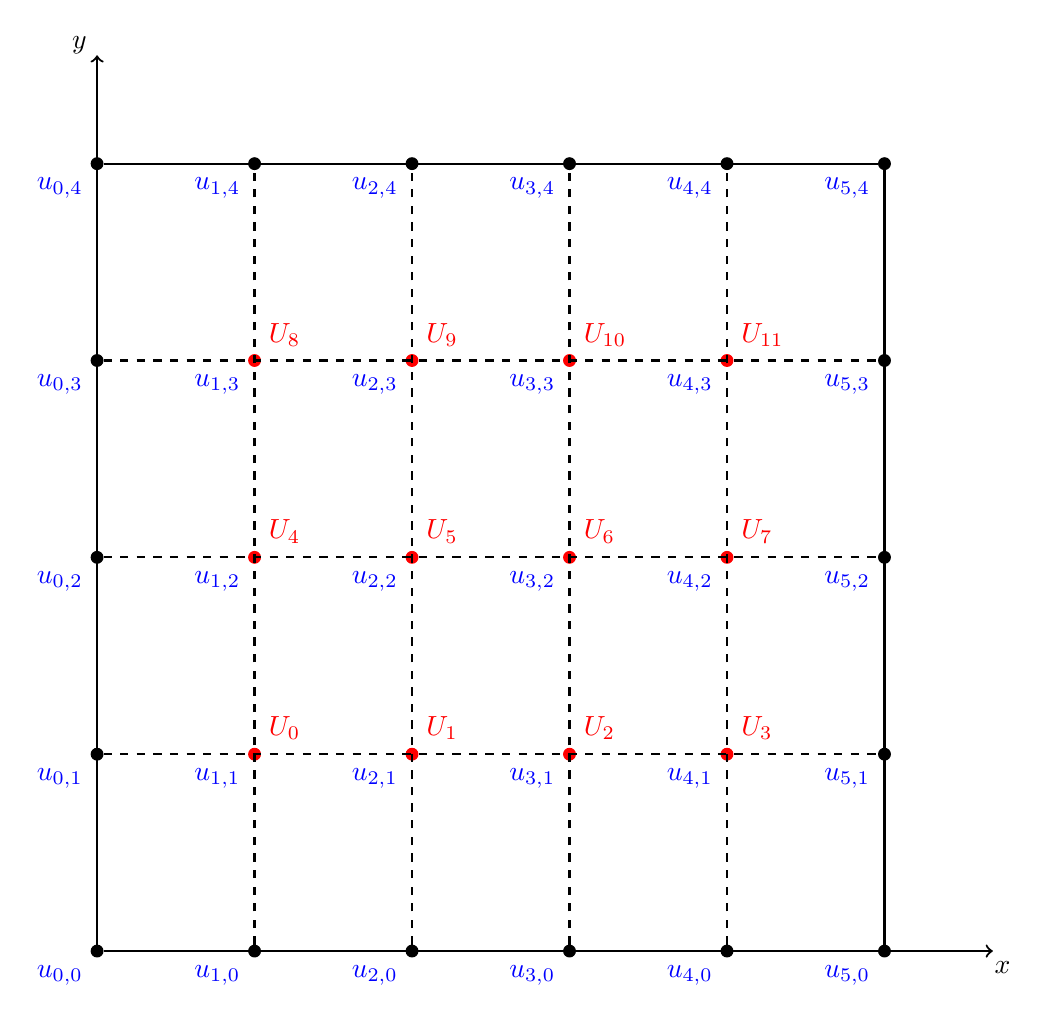
\begin{tikzpicture}[scale=1, , every node/.style={transform shape},
vertex/.style={circle, draw, fill, color=black, inner sep=1.5pt}]

\node[vertex, label={[blue]below left:$u_{0,0}$}] (1) at   (00.,00.0)     {};
\node[vertex, label={[blue]below left:$u_{0,1}$}] (2) at   (00.,02.5)     {};
\node[vertex, label={[blue]below left:$u_{0,2}$}] (3) at   (00.,05.0)     {};
\node[vertex, label={[blue]below left:$u_{0,3}$}] (4) at   (00.,07.5)     {};
\node[vertex, label={[blue]below left:$u_{0,4}$}] (5) at   (00.,10.0)     {};
\node[]       (5bis) at(00.,11.5)     {};
\node[vertex, label={[blue]below left:$u_{1,0}$}] (6) at   (02.,00.0)     {};
\node[vertex, red, label={[blue]below left:$u_{1,1}$}, label={[red]above right:$U_{0}$}] (7) at   (02.,02.5)     {};
\node[vertex, red, label={[blue]below left:$u_{1,2}$}, label={[red]above right:$U_{4}$}] (8) at   (02.,05.0)     {};
\node[vertex, red, label={[blue]below left:$u_{1,3}$}, label={[red]above right:$U_{8}$}] (9) at   (02.,07.5)     {};
\node[vertex, label={[blue]below left:$u_{1,4}$}] (10) at  (02.,10.0)     {};
\node[vertex, label={[blue]below left:$u_{2,0}$}] (11) at  (04.,00.0)     {};
\node[vertex, red, label={[blue]below left:$u_{2,1}$}, label={[red]above right:$U_{1}$}] (12) at  (04.,02.5)     {};
\node[vertex, red, label={[blue]below left:$u_{2,2}$}, label={[red]above right:$U_{5}$}] (13) at  (04.,05.0)     {};
\node[vertex, red, label={[blue]below left:$u_{2,3}$}, label={[red]above right:$U_{9}$}] (14) at  (04.,07.5)     {};
\node[vertex, label={[blue]below left:$u_{2,4}$}] (15) at  (04.,10.0)     {};
\node[vertex, label={[blue]below left:$u_{3,0}$}] (16) at  (06.,00.0)     {};
\node[vertex, red, label={[blue]below left:$u_{3,1}$}, label={[red]above right:$U_{2}$}] (17) at  (06.,02.5)     {};
\node[vertex, red, label={[blue]below left:$u_{3,2}$}, label={[red]above right:$U_{6}$}] (18) at  (06.,05.0)     {};
\node[vertex, red, label={[blue]below left:$u_{3,3}$}, label={[red]above right:$U_{10}$}] (19) at  (06.,07.5)     {};
\node[vertex, label={[blue]below left:$u_{3,4}$}] (20) at  (06.,10.0)     {};
\node[vertex, label={[blue]below left:$u_{4,0}$}] (21) at  (08.,00.0)     {};
\node[vertex, red, label={[blue]below left:$u_{4,1}$}, label={[red]above right:$U_{3}$}] (22) at  (08.,02.5)     {};
\node[vertex, red, label={[blue]below left:$u_{4,2}$}, label={[red]above right:$U_{7}$}] (23) at  (08.,05.0)     {};
\node[vertex, red, label={[blue]below left:$u_{4,3}$}, label={[red]above right:$U_{11}$}] (24) at  (08.,07.5)     {};
\node[vertex, label={[blue]below left:$u_{4,4}$}] (25) at  (08.,10.0)     {};
\node[vertex, label={[blue]below left:$u_{5,0}$}] (26) at  (10.,00.0)     {};
\node[]       (26bis) at(11.5,0.)     {};
\node[vertex, label={[blue]below left:$u_{5,1}$}] (27) at  (10.,02.5)     {};
\node[vertex, label={[blue]below left:$u_{5,2}$}] (28) at  (10.,05.0)     {};
\node[vertex, label={[blue]below left:$u_{5,3}$}] (29) at  (10.,07.5)     {};
\node[vertex, label={[blue]below left:$u_{5,4}$}] (30) at  (10.,10.0)     {};

\draw[thick, ->] (1) -- (5bis) node[left]{$y$};
\draw[thick, dashed] (6) -- (10);
\draw[thick, dashed] (11) -- (15);
\draw[thick, dashed] (16) -- (20);
\draw[thick, dashed] (21) -- (25);
\draw[thick] (26) -- (30);
\draw[thick, ->] (1) -- (26bis) node[below]{$x$};;
\draw[thick, dashed] (2) -- (27);
\draw[thick, dashed] (3) -- (28);
\draw[thick, dashed] (4) -- (29);
\draw[thick] (5) -- (30);

\end{tikzpicture}
 
\end{figure}

On a : 
\begin{eqnarray}
  x = x_{min} + i*\Delta x \, \\
  y = y_{min} + j*\Delta y \, \\
  I = (j-1)*Ny + (i-1) [TODO]
\end{eqnarray}

L'équation 
\begin{equation}
	\partial_t u - \sigma \Delta u = f
\end{equation}
se discrétise sous la forme suivante, dans le cas d'un schéma en temps d'Euler explicite et d'une discrétisation centrée d'ordre 1 en espace:
\begin{equation}
  \frac{u^{n+1}_{i,j}-u^{n}_{i,j}}{\Delta t} + \sigma \frac{2u^{n}_{i,j}-u^{n}_{i+1,j}-u^{n}_{i-1,j}}{\Delta x^2} + \frac{2u^{n}_{i,j} - u^{n}_{i,j+1} - u^{n}_{i,j-1}}{\Delta y^2} = f^{n}_{i,j}
\end{equation}


\end{document}
